\chapter{Constructing a control group}\label{ch:randomisation}

\section{A made-up example}\label{sec:beispiel}
Imagine that a new self-learning method for fostering
Danish reading skills in speakers of German has been developed.
You're tasked with finding out if this new method works
better than the old one.

\paragraph{First attempt} 
You find four students of German philology
who want to learn Danish. You ask them to work
autonomously with the new learning method
half an hour a day for three weeks. After three weeks,
you give them an article from a Danish newspaper,
which they are to summarise orally in German.
Two raters judge these summaries at their own discretion
(20-point scale); the mean of the two ratings per
learner counts as their reading comprehension score.
The average group score is 11/20.\\
What can you conclude from this study?

The answer is `pretty much nothing'.
One of several problems with this study is that 
there is no baseline against which to compare the participants'
average result: We don't know whether 11/20 indicates that the
new learning method works better or worse than the old one, or whether
the old and new learning methods are roughly equally effective.
So we need a comparison or \term{control group}
of people that didn't take part in the intervention.

\paragraph{Second attempt}
You convince four law students to also take part in the study.
They're asked to work with the old learning method
half an hour a day for three weeks.
Then they take the same test as the German philology students.
Their group mean is 8/20.\\
What can you conclude from this study?

\clearpage

\section{Critical questions}\label{sec:validitaet}%\cite{Nunan1992}\cite{Abbuhl2013}}

The second attempt outlined above also falls short on a number of criteria.
There are a couple of critical questions we can ask, and slightly modified
versions of these questions can be asked about studies in general.

\begin{description}
 \item[Internal validity]
 Can the difference in test scores between the two groups
 be ascribed to the difference in learning methods,
 or do alternative explanations for it present themselves?

 \item[External validity]
 Does the finding apply only to the present \term{sample}
 or can it be generalised to a larger \term{population}?
 To what population, exactly?

 \item[Ecological validity]
 (Especially for applied research.)
 To what extent are the findings applicable
 to the world outside of the lab
 (e.g., teaching, policy)?
 
 \item[Reliability]
  Are the raw data open for interpretation?
 
 \term{Inter-rater reliability}: Would different observers agree on the measurements?
 
 \term{Intra-rater reliability}: Would the \emph{same} observers agree on the measurements if they had to redo them?
 
  \item[Interpretative consensus]
  I use this non-standard term to refer to the possible problem captured
  by the following question:
 Confronted with the same data, would other researchers draw similar conclusions?

 \item[Replicability]
 Can the results of this study be confirmed
 in an independent \term{replication},
 that is, in a new but otherwise similar study?
\end{description}

\mypar[Ecological validity]{Example}
  Neurolinguistic research may show that using a foreign language highlights
  different brain regions in early and late learners.
  This may be interesting to neurolinguists.
  But for language policy, what's more relevant is the extent to which
  these groups differ behaviourally on communicatively relevant tasks.
\parend

\mypar[Interpretative consensus]{Example}
A study with considerable internal, external and ecological validity could show
that beginning L2 French learners vastly prefer using a rising intonation 
over other strategies
for formulating questions, but that more seasoned learners show a more balanced
use of the different strategies (subject--verb inversion, \textit{est-ce que}). 
Researchers may agree on these results, 
but are bound to disagree on which implications, 
if any, they ought to have for L2 French teaching. 

Generally, empirical findings obtained in basic research cannot be used
as evidence for nor against some teaching or learning method.
Such evidence must stem from targeted studies comparing teaching or learning
methods.
\parend
\medskip

The labels above aren't important; the questions behind them are.
Further, the questions asked above can rarely be answered in absolute terms.

\mypar{Exercise}
The second attempt outlined on page \pageref{sec:beispiel} is deficient 
in several of these respects. Discuss a few problems.
\parend

\begin{framed}
 Anticipate and resolve problems
related to lacking validity and reliability
\emph{before} collecting the data. This often
involves making compromises or coming to the
realisation that you can't satisfactorily
answer all your questions in a single study.
Do \emph{not} assume that some statistical method
will solve your problems.
\end{framed}

Depending on your goals, some types of validity
may not be as important as others.
For instance, for most studies in psycholinguistics,
university students are recruited as participants,
and their results don't necessarily generalise
to the population at large. But the purpose of these
studies is often to demonstrate that some
experimental manipulation \emph{can} affect
language use and processing, not that
it will affect language use in all language users.
From this perspective, these studies' lack
of external validity isn't too damning \citep{Mook1983}.

\mypar{Exercise}
  Skim the article by \citet{Offerman2016}
  and answer the following questions.
  
  \begin{enumerate}
    \item The study features two \term{conditions}:
    an experimental group and a control group.
    Briefly describe the difference between these conditions in terms
    of what the participants were asked to do. (Sections 3.1 and 3.3.)
    
    \item Consider the first research question on p.~48:
    ``Does a visual feedback paradigm improve production of the segmental
    feature voice onset time?''
    
    Based on your answer to the previous question, complete the following:
    
    ```Does a visual feedback paradigm improve production of the segmental
    feature voice onset time compared to [\textsc{your answer}]?''
    
    What would a stronger baseline for the comparison look like, and why?
    
    \item Who were the participants to this study? 
    Do the authors report how the participants were assigned to the study's
    conditions? (Section 3.1.) 
    
    How does this affect our (i.e., the readers') ability to judge the study's
    internal validity?
    \parend
  \end{enumerate}
  
  
\mypar{Exercise}
  \citet{DeWilde2020} found that Flemish children already knew
  a decent number of English vocabulary items even before they took their
  first English class.
  Especially English words similar in both form and meaning to their 
  Dutch translations (i.e., cognates) tended to be commonly known among
  these children.
  In their conclusion, the authors write that
  ```[t]he study also suggests that (\dots) teachers do not need to pre-teach
  some cognate words, even for learners at an elementary level'' (pp.~374--375).
  
  \citet{DeWilde2020} didn't empirically investigate the effects of implementing
  this suggestion. But can you think of an undesirable consequence
  of not `pre-teaching' English words with true Dutch cognates
  but still teaching false friends, i.e., English words for which a Dutch
  word with a similar form but a different meaning exists 
  (e.g., \textit{room}, which means `cream' in Dutch)?
\parend

\section{Increasing internal validity through randomisation}
Of the three types of validity considered, 
internal validity is the most pressing one:
If internal validity is low, external and ecological validity are both
essentially irrelevant.
Hence,
our first priority is to maximise the study's internal validity, that is,
we want to maximise the chances that any association we find in the data
can be ascribed to the factor of interest.
Confounding in particular represents a substantial threat to internal validity:
As we've seen in Chapter \ref{ch:causality}, confounding variables induce
associations between the variables of interest even in the absence of a causal
link between them. Moreover, even if a causal link does exist between the
variables of interest, confounding variables can bias the association
between them: The association may systematically under- or overestimate the
strength of the causal link. Keeping confounding in check is therefore key.

Your first inclination may be to try to ensure that the intervention and
control groups are identical in all respects save for the treatment itself.
That way, any differences in the outcome variable can't be explained by
confounding due to pre-existing differences between the groups.
However, it is practically
impossible to assign a fixed number of participants to two groups in such a
way that these groups are identical in all respects even in the utterly
unrealistic case where all the relevant information is available beforehand.
Clearly, it's entirely impossible to do so when not all of the relevant information
is available beforehand.

The solution is to assign the participants 
to the study's conditions \term{at random}, i.e., to deliberately leave the allocation
up to chance and chance alone. The \textsc{dag}s in Figure \vref{fig:randomisation} show what such
randomisation achieves. When the participants themselves (or their parents,
or their circumstances, etc.) decide or otherwise affect which condition they end up in ($X$),
confounding is a genuine concern (left).
However, when we assign the participants to the conditions at random,
we \emph{know} that there is no systematic link between pre-existing characteristics
($U$) and $X$, let alone a causal one. That is, randomisation prevents any
causal arrows from entering $X$ (right)! The result of this is that the
non-causal path between $X$ and $Y$ (via $U$) is broken and that the $X$-$Y$
relationship is no longer confounded by $U$.
To highlight that the values of $X$ were specified at random,
we use a subscript $_r$.

Studies in which the participants
are randomly assigned are called \term{true experiments}.
Random allocation by itself doesn't guarantee that the results of the
experiment can be trusted or interpreted at face value, but it does eliminate
confounding as a threat to the study's internal validity.

\begin{framed}
 Randomise wherever possible -- unless you have a \emph{very} good reason not to!
\end{framed}

\begin{figure}[tbp]
    \centering
    \begin{minipage}{0.45\textwidth}
        \centering
        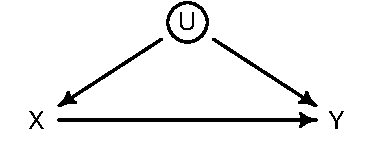
\includegraphics[width=\textwidth]{figure/w_o_randomisation}
    \end{minipage}\hfill
    \begin{minipage}{0.45\textwidth}
        \centering
        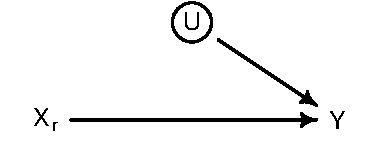
\includegraphics[width=\textwidth]{figure/w_randomisation}
    \end{minipage}
    \caption{\textit{Left:} The $X$-$Y$ relationship is confounded by $U$: there are two paths from $X$ to $Y$, but only one causal one.
    \textit{Right:} Randomising the values of $X$ prevents arrows from $U$ entering $X$, which effectively closes the non-causal path
    via the confounder.}
    \figlabel{fig:randomisation}
\end{figure}

\mypar{Tip}
  When reading empirical research articles, always look up if and how
  the participants (or classes, or whatever is of interest) were assigned
  to the study's conditions.
  And unless it explicitly says that the assignment was carried out at
  random, do not assume that it was.
\parend

\subsection{Why experiments?}
 \begin{enumerate}
  \item ``Experiments allow us to set up a \textbf{direct comparison} between the treatments of interest.
  \item ``We can design experiments to \textbf{minimize any bias} in the comparison. [especially randomisation]
  \item ``We can design experiments so that the \textbf{error} in the comparison is \textbf{small}. [see later chapters]
  \item ``Most important, we are \textbf{in control} of experiments, and having that control allows us to make stronger inferences about the nature of differences that we see in the experiment. Specifically, we may make \textbf{inferences about causation}.'' \citep[p.~2, my emphasis]{Oehlert2010}
 \end{enumerate}

What's meant by the first point is that we don't need to piece together snippets of evidence
from different and often difficult-to-reconcile sources (e.g., in a literature review) to figure
out which treatment (e.g., which learning method) works best in some situation.
Instead, we set up an experiment that directly evaluates the efficacy of several treatments
in the context we're interested in.

The second point alludes to techniques such as randomisation; the third to techniques
that we will encounter in the chapters to come.

\subsection{What does randomisation do?}
\begin{enumerate}
 \item ``Randomization balances the population on average.''
 \item ``The beauty of randomization is that it helps prevent confounding, \emph{even
for factors that we do not know are important}.'' \citep[p.~15, my emphasis]{Oehlert2010}
\end{enumerate}

We've already discussed the second point, 
but the first point warrants some explanation.
Some fundamental results from combinatorics are useful at this stage.

\mypar{Lemma}\label{lemma:permutations}
  If you have $n \geq 0$ distinct objects,
  there are 
  \begin{align*}
    \begin{cases}
      n(n-1)\cdots 2 \cdot 1, & \textrm{if $n \geq 1$}, \\
      1, &\textrm{if $n = 0$.}
    \end{cases}
  \end{align*}
  different ways to sort them (`\term{permutations}').
\parend

\begin{proof}\marginnote{This script includes a few proofs. You don't have
to learn them as such (I won't ask for proofs on the exam), but do try to 
understand them. The reason why I included them is that these proofs 
help to demystify what might otherwise seem to be arbitrary pronouncements.
Further, these proofs clarify exactly which assumptions a claim depends on 
and how far it extends: a proof can show you that an argument holds regardless 
of some detail that you might otherwise have assumed was essential to it.}
  If $n = 0$, there is only one way to sort the objects: do nothing.

  If $n \geq 1$: There are $n$ candidates to fill the first slot.
  Once a candidate for the first slot has been picked,
  $n-1$ candidates remain for the second slot, and so on,
  till there is only a single candidate left for the final slot.
\end{proof}

\mypar[Factorial]{Definition}
  For any natural number $n$, we define
  \begin{align*}
    n! :=     
    \begin{cases}
      n(n-1)\cdots 2 \cdot 1, & \textrm{if $n \geq 1$}, \\
      1, &\textrm{if $n = 0$.}
    \end{cases}
  \end{align*}
  We say `$n$ \term{factorial}' for `$n!$'.
\parend

\mypar{Lemma}
	There are
  \begin{align*}
    \frac{n!}{k!(n-k)!}
  \end{align*}
  different ways to choose $k \geq 0$ objects from among $n \geq k$
  distinct objects.
\parend

\begin{proof}
  With Lemma \ref{lemma:permutations}, there are $n!$ ways to arrange the $n \geq 0$ distinct objects.
  For each possible rearrangement, pick the first $k$ objects.
  This covers all possible choices of $k$ from $n$ objects.
  However, several rearrangements result in the same selection.
  Specifically, if we rearrange the first $k$ elements and the last $n-k$
  elements separately from each other, we end up with the same selection:
  the order among the first $k$ and among the last $n-k$ doesn't matter.
  Hence, again with Lemma \ref{lemma:permutations}, there are, for each of the $n!$ permutations,
  $k!(n-k)!$ rearrangements that result in the same selection.
  So there are $\frac{n!}{k!(n-k)!}$ different possible selections.
\end{proof}

\mypar[Binomial coefficient]{Definition}
  For natural numbers $n$ and $k$ with $n \geq k$, we define
  \[
    {n \choose k} := \frac{n!}{k!(n-k)!}.
  \]
  A term of this form is called a
  \term{binomial coefficient};
  we say `$n$ choose $k$' for `${n \choose k}$'.\marginnote{The binomial coefficient is called so because these terms
  appear when expanding binomial expressions such as $(a + b)^n$. 
  In German, one usually says `$n$ tief $k$' or `$k$ aus $n$' for $n \choose k$; 
  in French, `$k$ parmi $n$'.}
\parend
\medskip







